\documentclass[]{standalone}
\usepackage[utf8]{inputenc}
\usepackage[american]{circuitikz}
\usetikzlibrary{arrows,shapes,calc,positioning}

\usepackage{graphicx}

\newcommand{\myscope}[2] % #1 = name , #2 = rotation angle
{\draw[thick,rotate=#2] (#1) circle (12pt)
 (#1) ++(-0.35,-0.1) -- ++(0.3,0.3) --++(0,-0.3)-- ++(0.3,0.3) --++(0,-0.3);
}

\begin{document}

\pgfmathsetmacro\circuitheight{8}
\pgfmathsetmacro\circuitwidth{11}

\begin{circuitikz}[scale=1]
  % Power rails
  \draw (0,0) to[V, label=18V] (0, \circuitheight) to[short, -o] ++(\circuitwidth, 0); 
  \draw (0,0) to [short, -o] ++(\circuitwidth, 0); 


  \begin{scope}[xshift=8cm, yshift=2cm]
    \node at (0,0) {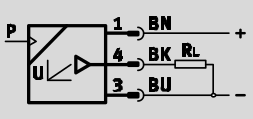
\includegraphics[width=3cm]{pressure-transmitter.png}};
    \node[coordinate] (psplus) at (1.2,.3) {};
    \node[coordinate] (psmin) at (1.2,-.4) {};
    \node[coordinate] (pssignal) at (2.6,-0.05) {};
    \draw (pssignal) to [short, -*] ++(-1.6,0);
  \end{scope}
  \draw (psplus |- 0,\circuitheight) to [short,-*] (psplus);
  \draw (psmin |- 0,0) to [short,-*] (psmin);
  \draw (pssignal |- (0,0) to[sV, color=white, name=S] (pssignal);
  \myscope{S}{0}

  \begin{scope}[xshift=6.5cm, yshift=6cm]
    \node[draw, minimum width=2cm, minimum height=1.6cm] (valve) at (0,0) {Valve};
    \node[coordinate, ] (vplus) at (-1.4, 0.6) {}; 
    \draw (valve.west |- vplus)  to [short, -*, color=red] (vplus);
    \node[coordinate, ] (vmin) at (-1.4, -0.6) {}; 
    \draw (valve.west |- vmin)  to [short, -*, color=blue] (vmin);
    \node[coordinate, ] (vwhite) at (-2.4, -0.2) {}; 
    \draw (valve.west |- vwhite)  to [short, -o] (vwhite);
    \node[coordinate, ] (vblack) at (-2.4, 0.2) {}; 
    \draw (valve.west |- vblack)  to [short, -*] (vblack);

  \end{scope}
  \draw (vplus |- 0,\circuitheight) to [short,] (vplus);
  \draw (vmin |- 0,0) to [short,] (vmin);
  \draw (vwhite |- 0,0) to [short,] (vwhite);
  
  \draw (3,0) to[sqV, label={} ] (3,0 |- vblack) to[short] (vblack);

  \node[coordinate, left of=vblack, node distance=2.5cm] (Osc) {};
  \draw (vblack) to[short] (Osc) to[sV, color=white, name=S2] (Osc |- 0,0);
  \myscope{S2}{0}
\end{circuitikz}
\end{document}
